\chapter{Uvod}

\qquad U ovom radu je predstavljeno upravljanje električnim vozilom (slika \ref{fig:buggy}) sa pogonom na sva četiri točka. Proizvođač \href{https://www.qsmotor.com/product/8000w-car-motor/}{motora} je kompanija \textit{QSMOTOR}. Snaga motora je $8000W$, a standardni napon napajanja iznosi $72V$. Svaki od motora je spojen na odgovarajući pretvarač/\href{https://kellycontroller.com/shop/kls-h/}{invertor}. Motori su trofazni i sadrže dva seta Hallovih senzora za određivanje brzine i pozicije. Datasheet motora je dat u prilogu \ref{motor_datasheet}, a dio dokumentacije pretvarača \textit{KLS7275H} u prilogu \ref{kelly_datasheet}. Razvoj upravljačkog prototipa će biti realiziran pomoću \href{https://www.dspace.com/en/inc/home/products/hw/microlabbox.cfm?fbclid=IwAR08_hHwsXPVRs6ng2DLSU5HA3vDNzpBa9CMpO8DWlSQ1DXPK58BkLmoiRE}{dSpace} sistema.

\begin{figure}
\begin{center}
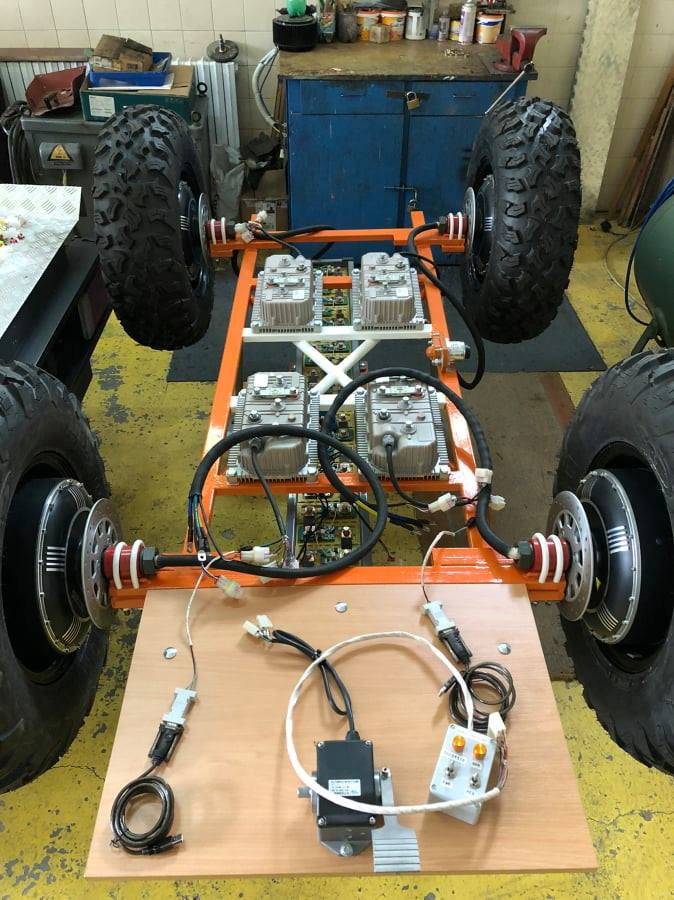
\includegraphics[scale=0.5]{slike/electric_car.jpg}
\end{center}
\caption{Električno $4x4$ vozilo}
\label{fig:buggy}
\end{figure}

\section{Motor}

\qquad Motor je trofazni sa $16$ pari polova, nominalne snage $8000W$. Za mjerenje brzine i pozicije motora, dostupna su dva seta Hallovih senzora. Moguće je mjeriti i temperaturu motora pomoću temperaturnog senzora $KTY83/122$. Motor sadrži dva konektora, čiji pinovi odgovaraju pinovima na \textit{DJ7061Y-2.3-21} konektoru energetskog pretvarača. Svaki od konektora daje informacije sa Hallovog i temperaturnog senzora.

\section{Pretvarač}

\qquad Energetski pretvarač \textit{KLS7275H} proizvođača \textit{Kelly} sadrži 5 digitalnih ulaza: prekidače za gas i kočnicu, prekidače za kretanje naprijed i nazad, te prekidač za \textit{boost} način rada. Dostupna su 3 analogna ulaza: gas, kočnica i temperatura motora. Opseg ulaznog napona može varirati od $0$ do $5V$. Za upravljanje je moguće koristiti i palicu (\textit{engl. joystick}), pri čemu pozicija palice određuje zadanu brzinu i smjer kretanja. \textit{Cruise} režim rada, koji je također dostupan, podrazumijeva zadržavanje zadane brzine vrtnje motora sve dok se ne zada nova brzina ili aktivira kočnica. Pretvarač podržava povezivanje putem \textit{CAN} mreže.

\subsection{Pinovi energetskog pretvarača}

\qquad \textit{KLS7275H} kontroler posjeduje tri konektora prikazana na slici (\ref{fig:kellypins} i 22 pina. Pored standardnih pinova za napajanje, pretvarač posjeduje pinove za prikupljanje informacija sa motora (Hallov senzor i temperaturni senzor), kao i pinove za definiranje smjera i brzine vrtnje motora. Žica spojena na odgovarajući pin je označena jedinstvenom bojom i brojem. Funkcije pinova su date u nastavku.

\begin{itemize}
	\item Konektor \textit{DJ7091Y-2.3-11}
	\begin{itemize}
		\item REV-SW (14) - prekidač za kretanje nazad
		\item GND (6) - minus napona napajanja, povratni signal
		\item FWD (12) - prekidač za kretanje naprijed
		\item 12V (11) - naponski izvor od $12V$
		\item 12V Brake (25) - ručna kočnica
		\item ECO (22) - prekidač za štedljivi način rada
		\item CAN-H (33) - \textit{high} pin za CAN komunikaciju
		\item PWR (7) - plus napona napajanja pretvarača
		\item CAN-L (34) - \textit{low} pin za CAN komunikaciju
	\end{itemize}
	\item Konektor \textit{DJ7091Y-2.3-21}
		\begin{itemize}
		\item FOOT-SW (15) - prekidač za gas
		\item Throttle (3) - analogni ulaz za gas ($0-5V$)
		\item GND (20) - minus napon napajanja, povratni signal
		\item Meter (8) - kopija signala sa Hallovog senzora
		\item 5V (4) - naponski izvor od $5V$
		\item Brake-AN (2) - \textit{boost} funkcija ili analogni ulaz za regenerativni tip kočenja
		\item 12V (11) - naponski izvor od $12V$
	\end{itemize}
	\item Konektor \textit{DJ7061Y-2.3-21}
		\begin{itemize}
		\item GND (21) - minus napon napajanja, povratni signal
		\item Temp (1) - temperatura motora
		\item 5V (5) - naponski izvor od $5V$
		\item Hall A (18) - signal Hallovog senzora za fazu A
		\item Hall B (17) - signal Hallovog senzora za fazu B 
		\item Hall C (16) - signal Hallovog senzora za fazu C 
	\end{itemize}
\end{itemize}

\begin{figure}[]
\begin{center}
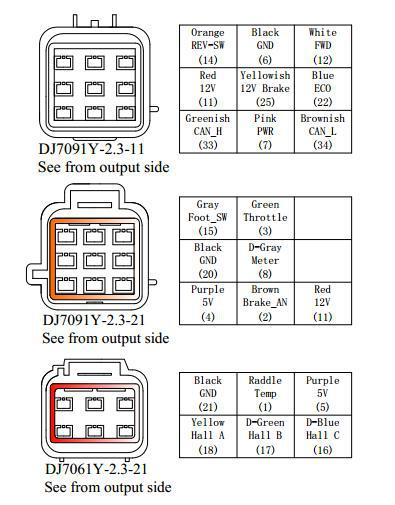
\includegraphics[scale=1]{slike/kellypins.jpg}
\end{center}
\caption{Pinovi \textit{Kelly KLS7275H} pretvarača}
\label{fig:kellypins}
\end{figure}










